\documentclass{uonmathreport}

% loads already mathtools, graphicx,
% but you may want to add other packages, like
\usepackage{listings} % to include code in python see https://en.wikibooks.org/wiki/LaTeX/Source_Code_Listings
\usepackage{xcolor}
\usepackage{biblatex}
\addbibresource{progress.bib}
% other useful pagackes include booktabs, hyperref, amsthm, xcolor, todonotes, showkeys, ...
% see https://www.overleaf.com/learn 

% change the following to
% to \PJA = MATH4041, \PJS = MATH4042 or \DIS = MATH4001 (for BSc and MMAth)
% or \MSc (for all Msc dissertations)
\PJA

% adjust the following
\title{Title of the report goes here\\ and it may have several lines}
\author{Alvin Jonel De la Cruz Guerrero}
\academicyear{2022/23}
\supervisor{Dr. Your Supervisor}

% the following are irrelevant for Msc:
\assessmenttype{Review} % or Investigation

% the following are irrelevant for PJS, PJA, DIS:
% Msc: change it to G14PMD and Pure Mathematics, etc ...
\msccode{MATH4021}
\msctitle{Statistics}

% put your own definitions and shorthands here
\newcommand{\ZZ}{\mathbb{Z}}

\begin{document}

\maketitle

\begin{abstract}
The abstract of the report goes here. The abstract should state the
topic(s) under investigation and the main results or
conclusions. Methods or approaches should be stated if this is
appropriate for the topic. The abstract should be self-contained,
concise and clear. The typical length is one paragraph.
\end{abstract}

% Table of contents
\setcounter{tocdepth}{3}  % this will list subsections, but not subsubsections
\tableofcontents 
\newpage
% this is a comment in the file that won't appear in the output


\section{Introduction}

\subsection{Overview}

Options are equity-based derivatives that are primarily used to mitigate risk. The options market is significantly larger compared to other derivatives. In fact, options were the most traded derivatives in 2019, with a volume of 18.55 billion contracts when combining index and individual equities contracts\cite{statista_2019}. An enormous market like the options market demands reliable pricing mechanisms to minimize arbitrage opportunities. Naturally, pricing American options is a broad research area because there is no closed-form solution to the PDE resulting from the Black-Scholes model. Merton\cite{merton_1973} was the first to consider the Black-Scholes\cite{black_scholes_1973} model to price European and American options. Although Merton derived a nice formula to price European options, he stated that, in general, a closed-form solution was not attainable for American options. In 1977, Schwartz\cite{schwartz_197779} and Brennan\cite{brennan_1997} proposed using finite difference schemes to solve the pricing problem for American options. The work of Merton and Schwartz served as a foundation for the free boundary problem formulation of the pricing problem. The motivation behind the free boundary problem formulation is that for American options, there exists an optimal exercise price that marks the boundary between the region where exercising the option is profitable and the region where it is not. Moreover, this optimal exercise price changes with time, making it impossible for the holder to determine when to exercise. Based on the work of Landau\cite{landau_1950_heat_ci}, Wu et al.\cite{wu1997front} formulated the front-fixing method as an approach to solve the free boundary problem for options, in which the Landau transformation is used to transform the moving boundary into a fixed boundary. Multiple transformations have been proposed by Huang et al.\cite{huang_2000}, Nielsen et al.\cite{nielsen_2001}, and Company et al.\cite{company_egorova_jodar_2014}. Around the same period, Dewynne et al.\cite{dewynne_howison_rupf_wilmott_1993} took a different approach to solve the pricing problem. The idea was to reformulate the free boundary problem as a problem with variational inequalities that, when finite difference is applied, transforms into a linear complementary problem\cite{cottle_1968}.

\subsection{Aim} 

The goal of this work is to implement the numerical methods proposed by Nielsen et al.\cite{nielsen_2001} and Company et al.\cite{company_egorova_jodar_2014} to solve the free boundary formulation of the pricing problem for American options\cite{dewynne_howison_rupf_wilmott_1993}. Moreover, Company et al.\cite{company_egorova_jodar_2014} and Nielsen et al.\cite{nielsen_2001} proposed schemes for pricing American put options with underlying assets that have non-paying dividends. However, we aim to derive analogous schemes for pricing call contracts, and consider underlying assets that have a continuous dividend yield, such as the S\&P500.  Furthermore, we consider the PSOR method proposed by Dewynne\cite{dewynne_howison_rupf_wilmott_1993}\cite{dewynne_howison_wilmott_howison_1995} to solve for the variational inequalities formulation of the pricing problem. Finally, we conduct a convergence analysis for each the schemes derived.

\subsection{Main Achievements}

In this work, we were able to derive the corresponding PDE problem resulting from applying the transformations proposed by Nielsen et al.\cite{nielsen_2001} and Company et al.\cite{company_egorova_jodar_2014} for call and put options with underlying assets featuring a continuous dividend yield. Moreover, we implemented explicit and implicit front fixing schemes for the Nielsen transformation method\cite{nielsen_2001}, an explicit front fixing scheme for Company transformation, and the theta PSOR scheme for the linear complementary problem proposed by Dewynne\cite{dewynne_howison_wilmott_howison_1995}. Finally, we derived the order of convergence for each of the implemented methods.

\subsection{Outline}

The outline of this paper is as follows. In section 2, we explore the Black-Scholes model for American options for assets that pay dividends, resulting in the free boundary formulation of the pricing problem. Furthermore, we delve into the front-fixing method as a strategy for fixing the moving boundary by applying the changes of variables proposed by Company et al.\cite{company_egorova_jodar_2014} and Nielsen et al.\cite{nielsen_2001}. In section 3, we explore explicit and implicit schemes to solve the partial differential equations resulting from applying the front-fixing method and the Nielsen transformation to the free boundary problem obtained in section 1. We conclude section 3 with numerical experiments and convergence analysis for the numerical schemes presented in section 3, and appendix \ref{sec:company_explicit_scheme}. In section 4, we explore a reformulation of the pricing problem as a variational inequality. Additionally, we derived the PSOR method as way to solve the linear complementary problem that arises from applying the theta method to the variational inequality. Finally, in the same section, we discuss the results obtained by explicit, implicit and Crank-Nicholson PSOR schemes.


\section{Black-Scholes equation} \label{sec:blackscholes}

\subsection{Preliminaries}

A common problem in finance is to price financial derivatives, often referred just
as derivatives. In essence, derivatives are contracts set between parties 
whose value in time derives from the price of their underlying assets. A notorious
family of derivatives in financial markets are "options". Options
are contracts set between two parties in which the holder has the right 
to sell or buy, commonly referred as exercise, an underlying stock at a preestablished price, 
also known as "strike price", in the future. Options are referred as "call options" 
or as "put options" if the exercise position is to buy or to sell, respectively. 
Similarly, options are classified depending on their exercise style. In that regard,
the simplest of options are European options. European options give the right 
to exercise at the expiration date of the contract. Another well known type options 
are American options. American options work similar as European options with the
difference that can be exercised at any point in time between the beginning and 
expiration date of the contract. 
Let us define the payoff as

\begin{subequations} \label{eq:blackscholes:preliminaries:payoff_function}
  \begin{equation}
    H(S,t) = \max(S - K, 0)
  \end{equation}  
  \begin{equation}
    H(S,t) = \max(K - S, 0)
  \end{equation}
\end{subequations}

where $K$ is the strike price, $S\in[0,\infty]$ is the stock price, and 
$t \in [0, T]$ is the current time. Note that $t$ is measure in years, $t=0$ and $t=T$
denotes the beginning of the contract and the expiration date, and
the region $[0,T]$ is the life span of the option. While an American option's payoff
is defined for all $(S,t)$, European options' payoff is only defined at $t=T$.   

Obviously, options give greater flexibility 
to holders by removing their exposure of a negative payoff which is why writers of 
the option charge a premium to the buyers at the time they enter the contract. 
The premium is often referred as the price or value of the option and the problem of finding this value is called option pricing. 
When pricing options, it is important to find the just price because 
otherwise the writer or buyer of the option could set some scheme in which option
will always be profitable to them. In other words, options pricing must follow
the principle of no-arbitrage. Therefore, we assume that the writer of the option
uses the premium to construct a portfolio consisting of $\phi_0$ units of the 
stock and invests $\psi_0$ units of cash into a risk-free asset such as US
treasury bill, certificate of deposit, or bank account. Then, the writer rebalanced
the portfolio $(\phi_0, \psi_0)$ to hedge any 
possible claims from the buyer of the option at any future time $0 < t \le T$. 
Therefore, at any time $t$, the writer holds a portfolio $(\phi(t), \psi(t))$ 
with value

\begin{equation}
  \Pi(t) = \phi(t)S(t) + \psi(t)B(t)
\end{equation}

Moreover, the portfolio is self-financing. In other words, the changes in the value
of the portfolio $V(t)$ depend on the changes in $S(t)$ and $B(t)$, and the current
portfolio $(\phi(t), \psi(t))$

\begin{equation}
  d\Pi(t) = \phi(t)dS(t) + \psi(t)dB(t)
\end{equation}

Finally, the value of an option must satisfy the following

\begin{equation}
  \Pi(t) = V(t)
\end{equation}

at any time $0 \le t \le T$.

The Black-Scholes model is built upon the self-financing portfolio hedging strategy 
and expresses a mathematical model for dynamics of option's price. 
The Black-Scholes model makes some assumptions about the market. For a complete
list of these assumptions look at (reference). We enumerate the one we believe 
are important for our task. First, the stock price $S(t)$ is a log-normal random
variable 

\begin{equation}
  dS = r(t)Sdt + \sigma(t) S dW
\end{equation}

where the risk-free interest $r(t)$ and the price volatility $\sigma(t)$ are 
deterministic functions of time during the life of the option. Secondly, the 
bank account $B(t)$ is a deterministic function of time

\begin{equation}
  dB = r(t)B(t)dt
\end{equation}

Finally, the stock does not pay dividends. From now on, we will assume that 
the risk-free interest rate and stock price volatility are constant during the 
life of the option. Later on, we will address the assumption about dividends.

By applying the Black-Scholes model to price European options, the famous Black-Scholes 
PDE is obtained

\begin{equation}
  \begin{cases}
    \dfrac{\partial{V}}{\partial{t}} + \dfrac{1}{2}\sigma^{2} S^2 \dfrac{\partial^2{V}}{\partial{S^2}} + r S \dfrac{\partial{V}}{\partial{S}} - rV = 0 & \text{for $t\in[0,T)$ and $S\in[0, \infty)$} \\
    V(S, T) = H(S, T) & \text{for $S\in[0, \infty)$}
  \end{cases}
  \label{eq:blackscholes:finance:european_option_pde}
\end{equation}

where $V(S, t)$ is a deterministic function. For the derivation of 
\eqref{eq:blackscholes:finance:european_option_pde}, we reference to REFERENCE.

We previously mention that the one of the assumptions of the Black-Scholes model is
that the underlying stock does not pay dividends. In most cases, assets such as stock
pay out dividends just a few times at year. Therefore, dividends are to be 
modelled discretely. However, there are certain assets that pay out a proportion
of the current asset price during and interval of time. Thus, in such cases, it is
useful to model dividends as a continuous yield. By arbitrage arguments [REFERENCES], it can be shown that the asset price with volatility $\sigma(t)$, rate of return $r(t)$,
and continuous dividend yield $\delta(S,t)$ paid at instant of time $dt$ is modeled as

\begin{align}
  dS = (r(t) - \delta(S, t))Sdt + \sigma(t) S dW
  \label{eq:blackscholes:finance:bs_price_model_with_dividends}
\end{align}

Similarly to
as we did for the risk-free interest rate and the volatility of the asset price,
we will assume that continuous dividends yield is as constant from now on. [REFERENCES]
show that applying the Black-Scholes model under the price model \eqref{eq:blackscholes:finance:bs_price_model_with_dividends} to price European options,
we obtain the slightly modified version of \eqref{eq:blackscholes:finance:european_option_pde}

\begin{equation}
  \begin{cases}
    \dfrac{\partial{V}}{\partial{t}} + \dfrac{1}{2}\sigma^{2} S^2 \dfrac{\partial^2{V}}{\partial{S^2}} + (r - \delta) S \dfrac{\partial{V}}{\partial{S}} - rV = 0 & \text{for $t\in[0,T)$ and $S\in[0, \infty)$} \\
    V(S, T) = H(S, T) & \text{for $S\in[0, \infty)$}
  \end{cases}
  \label{eq:chapter2:european_option_pde_with_dividens}
\end{equation}
 
Similarly, the Black-Scholes model is applied to price American options. 
One important result is that the value of an American option $V_\text{Ame}(t)$ is
bounded from below by the payoff function
\begin{align}
  V_{\text{Am}}(S, t) \ge H(S, t) \qquad \text{for $t\in[0,T]$}
  \label{eq:blackscholes:american_options_price_lower_bound}
\end{align}

Moreover, the domain of $V(S,t)$ can be separated in the exercise region 
\begin{equation}
  \mathcal{S} := \{(S, t): V(S, t) = H(S, t) \}
  \label{eq:background:finance:exercise_region}
\end{equation}

and the continuation region 
\begin{equation}
  \mathcal{C} := \{(S, t): V(S, t) > H(S, t) \}
\end{equation}

where the boundary of $\mathcal{C}$ is defined as

\begin{equation}
  \partial \mathcal{C} := \{(S, t): S = \bar{S}(t)\} 
  \label{eq:background:finance:exercise_region}
\end{equation}

Lastly, the price dynamics of American options behaves as European options within
the continuation region. Since we know $V(S, t)$ at the stopping region, we only
need to solve $V(S,t)$ at continuation region and determine its boundary $\partial$
at the same time. Therefore, this is known as the free boundary problem formulation
of the American option pricing problem and is equivalent to solve.
\begin{align}
  \begin{cases}
  \dfrac{\partial{V}}{\partial{t}} + \dfrac{1}{2}\sigma^{2} S^2 \dfrac{\partial^2{V}}{\partial{S^2}} + (r - \delta)S \dfrac{\partial{V}}{\partial{S}} - rV = 0 & \text{for $(S, t) \in \mathcal{C}$} \\
  V(S, t) = H(S, t) & \text{for $(S,t)\in \partial\mathcal{C}$}
  \end{cases}
  \label{eq:blackscholes:finance:american_options_pde_free_boundary_problem}
\end{align}

Since the holder of an American option would always at the expiration date $T$
exercise the if it is profitable or would not make a profit otherwise. Therefore,
American options value is equal to its payoff at the maturity date. With this 
information, we could establish terminal conditions for the free boundary problem 
in \eqref{eq:blackscholes:finance:american_options_pde_free_boundary_problem}.
\begin{align*}
  & V(S,T) = H(S, T) \\
  & \bar{S}(T) = K
\end{align*}

Next, we need to establish boundary conditions for the system 
\eqref{eq:blackscholes:finance:american_options_pde_free_boundary_problem}. 
Generally, when pricing options, we would need two boundaries conditions 
for option pricing. However, the free boundary problem in 
\eqref{eq:blackscholes:finance:american_options_pde_free_boundary_problem}
is expressed in terms on the moving boundary condition $\bar{S}(t)$. Therefore,
we only need to determine one extra boundary condition. In case of 
American put options, the left boundary condition would be given by $\bar{S}(t)$,
and the right boundary condition by $V(S, t) = 0$ for a sufficiently large $S$. 
Analogously, $\bar{S}(t)$ would be the right boundary condition for 
an American call option and its left boundary condition by $V(S, t) = 0$ for $S = 0$. 
Finally, one extra information is that at the point $(\bar{S}(t), t)$, the 
derivative of the value with respect to the price is given by:

\begin{subequations}
  \begin{equation}
    \dfrac{\partial{V}}{\partial{S}}(\bar{S}(t), t) = 1 \qquad \text{(call)}
  \end{equation}
  \begin{equation}
    \dfrac{\partial{V}}{\partial{S}}(\bar{S}(t), t) = -1 \qquad \text{(put)}
  \end{equation}
\end{subequations}

Grouping , boundary conditions and terminal condition 
in one equation, we obtain the system.

\begin{subequations} \label{eq:blackscholes:finance:american_options_pde_free_boundary_problem_full}
\begin{equation}
  \begin{cases}
    \dfrac{\partial{V}}{\partial{t}} + \dfrac{1}{2}\sigma^{2} S^2 \dfrac{\partial^2{v}}{\partial{x}^2} + (r - \delta)S\dfrac{\partial{V}}{\partial{S}} - rV = 0 & \text{for $0 \le S < \bar{S}(t)$ and $0 \le t < T$} \\
    V(S, T) = S - K \qquad \bar{S}(T) = K \\
    V(0, t) = 0 \quad \dfrac{\partial{V}}{\partial{S}}(\bar{S}(t), t) = 1
  \end{cases}
\end{equation}
\begin{equation}
  \begin{cases}
    \dfrac{\partial{V}}{\partial{t}} + \dfrac{1}{2}\sigma^{2} S^2 \dfrac{\partial^2{v}}{\partial{x}^2} + (r - \delta)S\dfrac{\partial{V}}{\partial{S}} - rV = 0 & \text{for $\bar{S}(t) < S < \infty$ and $0 \le t < T$} \\
    V(S, T) = K - S \qquad \bar{S}(T) = K \\
    \lim_{S\rightarrow\infty}V(S, t) = 0 \quad \dfrac{\partial{V}}{\partial{S}}(\bar{S}(t), t) = -1
  \end{cases}
\end{equation}

\end{subequations}

\subsection{Front-Fixing method}

In the previous section, we presented the pricing of American options problem.
By applying the Black-Scholes model, we derived the Black-Scholes PDE that describes 
the price dynamics in the continuation region $\mathcal{C}$ of call and put options.
Moreover, we presented the moving boundary condition $\bar{S}(t)$ for this PDE.
The moving boundary condition $\bar{S}(t)$ makes the Black-Scholes PDE more 
involved since we also need to determine this boundary as time changes. This type 
of problem are known as free boundary problems. The front fixing method
was first introduced by \cite{landau_1950_heat_ci} and is a strategy in which 
we define a map from the original domain to new domain where moving boundary
remains constant as time changes. In this section, we explore two transformation
based on the work of Nielsen and others \cite{nielsen_2001}, and the work of
Company and others \cite{company_egorova_jodar_2014}.

\subsubsection{Inverse transformation}

This method proposes the transformation 
\begin{equation}
    x = \dfrac{S}{\bar{S}(t)}
    \label{eq:blackscholes:frontfixingmethod:inversetransform}
\end{equation}

which maps the boundary of the continuation region $\partial C$ defined in 
\eqref{eq:background:finance:exercise_region} to the fixed boundary 
\begin{equation}
  \mathcal{\partial C}_x := \{(x, t): x = 1\} 
\end{equation}

which remain constant as t changes. Now, let us define the value $v(x,t)$ 
under this new map
\begin{equation}
  v(x, t) := V(S, t)
  \label{eq:blackscholes:frontfixingmethod:inversetransform:value_function}
\end{equation}

which fixes the moving boundary $\bar{S}(t)$ at $x=1$ when $S(t)$. Next, we compute
the partial derivatives of $V$ with respect of the partial derivatives of $v$ which
will allow us to rewrite the PDE in \eqref{eq:blackscholes:finance:american_options_pde_free_boundary_problem_full} 
with respect of \eqref{eq:blackscholes:frontfixingmethod:inversetransform:value_function}

\begin{align*}
  \dfrac{\partial{x}}{\partial{S}} &= \dfrac{1}{\bar{S}(t)} \\\\
  \dfrac{\partial{x}}{\partial{t}} &= -x\dfrac{\bar{S}'(t)}{\bar{S}(t)} \\\\
  \dfrac{\partial{V}}{\partial{S}} &= \dfrac{\partial{v}}{\partial{x}}\dfrac{\partial{x}}{\partial{S}} = \dfrac{1}{\bar{S}(t)}\dfrac{\partial{v}}{\partial{x}} \\\\
  \dfrac{\partial^2{V}}{\partial{S^2}} &= \dfrac{1}{\bar{S}(t)} \dfrac{\partial{x}}{\partial{S}} \dfrac{\partial^2{v}}{\partial{x^2}} = \dfrac{1}{\bar{S}(t)^2} \dfrac{\partial^2{v}}{\partial{x}^2} \\\\
  \dfrac{\partial{V}}{\partial{t}} &=  \dfrac{\partial{v}}{\partial{t}} + \dfrac{\partial{v}}{\partial{x}} \dfrac{\partial{x}}{\partial{t}} = \dfrac{\partial{v}}{\partial{t}} - x\dfrac{\bar{S}^\prime(t)}{\bar{S}(t)}\dfrac{\partial{v}}{\partial{x}}
\end{align*}

Substituting these partial derivatives in the Black-Scholes PDE given by \eqref{eq:blackscholes:finance:american_options_pde_free_boundary_problem_full},
we obtain the non-linear PDE
\begin{subequations} \label{eq:blackscholes:frontfixingmethod:american_options_pde}
  \begin{align}  
    \dfrac{\partial{v}}{\partial{t}} + \dfrac{1}{2}\sigma^{2} x^2 \dfrac{\partial^2{v}}{\partial{x}^2} + \bigg[(r - \delta) - \dfrac{\bar{S}^\prime(t)}{\bar{S}(t)}\bigg]x\dfrac{\partial{v}}{\partial{x}} - rv = 0 \quad & \text{for $x \in [0, 1)$ and $t \in [0, T)$}\\
    \dfrac{\partial{v}}{\partial{t}} + \dfrac{1}{2}\sigma^{2} x^2 \dfrac{\partial^2{v}}{\partial{x}^2} + \bigg[(r - \delta) - \dfrac{\bar{S}^\prime(t)}{\bar{S}(t)}\bigg]x\dfrac{\partial{v}}{\partial{x}} - rv = 0 \quad & \text{for $x > 1$ and $t \in (0, T]$}
  \end{align}  
\end{subequations}

Likewise, we rewrite the terminal condition as
\begin{subequations} \label{eq:blackscholes:frontfixingmethod:inversetransform:american_options_terminal_condition}
  \begin{equation}
    v(x, T) = \max(x\bar{S}(T) - K) = K \max(x - 1, 0) = 0
  \end{equation}
  \begin{equation}
    v(x, T) = \max(K - x\bar{S}(T)) = K \max(1 - x, 0) = 0
  \end{equation}
\end{subequations}

Note that $x$ is always less than one for put options. Analogously, $x$ is 
always greater than one for call options. Finally, we rewrite the boundary condition
given by the optimal exercise price $\bar{S}(t)$ as
\begin{subequations} \label{eq:blackscholes:frontfixingmethod:inversetransform:american_options_optimal_price_bc}
  \begin{equation}
    \dfrac{\partial v}{\partial x}(1, t) = 1
  \end{equation}  
  \begin{equation}
    \dfrac{\partial v}{\partial x}(1, t) = -1
  \end{equation}
\end{subequations}

and the boundary condition opposite to the optimal exercise price as  
\begin{equation} \label{eq:blackscholes:frontfixingmethod:inversetransform:american_option_opposite_bc}
  v(0, t) = 0
\end{equation} 

for both put and call options. In summary, by groping equations 
\eqref{eq:blackscholes:frontfixingmethod:american_options_pde},
\eqref{eq:blackscholes:frontfixingmethod:inversetransform:american_options_terminal_condition},
\eqref{eq:blackscholes:frontfixingmethod:inversetransform:american_options_optimal_price_bc},
and \eqref{eq:blackscholes:frontfixingmethod:inversetransform:american_options_optimal_price_bc},
we obtain the system
\begin{subequations}
\begin{equation}
  \begin{cases}
    \dfrac{\partial{v}}{\partial{t}} + \dfrac{1}{2}\sigma^{2} x^2 \dfrac{\partial^2{v}}{\partial{x}^2} + \bigg[(r - \delta) - \dfrac{\bar{S}^\prime(t)}{\bar{S}(t)}\bigg]x\dfrac{\partial{v}}{\partial{x}} - rv = 0 & \text{for $x \in (0, 1)$ and $t \in [0, T]$} \\
    v(x, T) = 0 \qquad \bar{S}(T) = K \\
    v(0, t) = 0 \quad \dfrac{\partial{v}}{\partial{x}}(1, t) = \bar{S}(t)
  \end{cases}
\end{equation}
\begin{equation}
  \begin{cases}
    \dfrac{\partial{v}}{\partial{t}} + \dfrac{1}{2}\sigma^{2} x^2 \dfrac{\partial^2{v}}{\partial{x}^2} + \bigg[(r - \delta) - \dfrac{\bar{S}^\prime(t)}{\bar{S}(t)}\bigg]x\dfrac{\partial{v}}{\partial{x}} - rv = 0 & \text{for $x > 1$ and $t \in [0, T]$} \\
    v(x, T) = 0 \qquad \bar{S}(T) = K \\
    \lim_{x\rightarrow\infty}v(x, t) = 0 \quad \dfrac{\partial{v}}{\partial{x}}(1, t) = -\bar{S}(t)
  \end{cases}
\end{equation}
\end{subequations}

\subsubsection{Log transformation}

In this section, we define the transformations
\begin{equation}
  x := \log \dfrac{KS}{\bar{S}(t)} \qquad v(x, t) := \dfrac{V(S, t)}{K}
\end{equation}

which maps the boundary $\partial \mathcal{C}$ to the region
\begin{equation}
  \partial{\mathcal{C}_x} := \{ (x, t): x = \log{K} \}  
\end{equation}

\newpage

Similarly to the previous section, we compute the partial derivatives of $v(x,t)$,
\begin{align*}
  \dfrac{\partial x}{\partial t} &= -\dfrac{\bar{S}'(t) }{\bar{S}(t)} \\\\
  \dfrac{\partial x}{\partial S} &= \dfrac{1}{S} \\\\ 
  \dfrac{\partial V}{\partial S} &= \dfrac{K}{S} \dfrac{\partial v}{\partial x} \\\\
  \dfrac{\partial^2 V}{\partial^2 S} &= \dfrac{K}{S^2}\dfrac{\partial^2 v}{\partial x^2} - \dfrac{K}{S^2} \dfrac{\partial v}{\partial x} \\\\
  \dfrac{\partial V}{\partial t} &= K \dfrac{\partial v}{\partial t} - K\dfrac{\bar{S}'(t)}{\bar{S}(t)}\dfrac{\partial v}{\partial x}
\end{align*}

Using the partial derivates, we rewrite the Black-Scholes PDE as follows
\begin{subequations}
  \begin{align}
      \dfrac{\partial v}{\partial t} + \dfrac{1}{2}\sigma^2\dfrac{\partial^2 v}{\partial x^2} + \bigg((r-\delta) - \dfrac{\sigma^2}{2} \bigg)\dfrac{\partial v}{\partial x} -\dfrac{\bar{S}'(t)}{\bar{S}(t)}\dfrac{\partial v}{\partial x} - rv = 0 \quad \text{for $x < \log{K}$ and $t \in [0, T)$} \\
      \dfrac{\partial v}{\partial t} + \dfrac{1}{2}\sigma^2\dfrac{\partial^2 v}{\partial x^2} + \bigg((r-\delta) - \dfrac{\sigma^2}{2} \bigg)\dfrac{\partial v}{\partial x} -\dfrac{\bar{S}'(t)}{\bar{S}(t)}\dfrac{\partial v}{\partial x} - rv = 0 \quad \text{for $x > \log{K}$ and $t \in [0, T)$}
  \end{align}
\end{subequations}

with terminal condition
\begin{subequations} \label{eq:blackscholes:frontfixingmethod:logtransform:american_options_terminal_condition}
  \begin{equation}
    v(x, T) = \max\bigg(\dfrac{e^x}{K} - 1, 0\bigg) = 0
  \end{equation}
  \begin{equation}
    v(x, T) = \max\bigg(1 - e^x, 0\bigg) = 0
  \end{equation}
\end{subequations}

\newpage

Next, we rewrite the boundary condition given by the optimal exercise price
\begin{subequations}
  \begin{equation}
    \dfrac{\partial v}{\partial x}(\log{K}, t) = \dfrac{\bar{S}(t)}{K} 
  \end{equation}
  \begin{equation}
    \dfrac{\partial v}{\partial x}(\log{K}, t) = -\dfrac{\bar{S}(t)}{K}
  \end{equation}
\end{subequations}

and the boundary condition opposite to the optimal exercise price
\begin{subequations}
  \begin{equation}
    \lim_{x\rightarrow-\infty} v(x, t) = 0
  \end{equation}
  \begin{equation}
    \lim_{x\rightarrow\infty} v(x, t) = 0
  \end{equation}
\end{subequations}

Finally, grouping equations together, we have the system
\begin{subequations}
  \begin{equation}
    \begin{cases}
      \dfrac{\partial v}{\partial t} + \dfrac{1}{2}\sigma^2\dfrac{\partial^2 v}{\partial x^2} + \bigg((r-\delta) - \dfrac{\sigma^2}{2} \bigg)\dfrac{\partial v}{\partial x} -\dfrac{\bar{S}'(t)}{\bar{S}(t)}\dfrac{\partial v}{\partial x} - rv = 0 \quad \text{for $x < \log{K}$ and $t \in [0, T)$} \\
      v(x, T) = 0 \qquad \bar{S}(T) = K \\
      \lim_{x\rightarrow-\infty} v(x, t) = 0 \quad \dfrac{\partial{v}}{\partial{x}}(\log{K}, t) = \dfrac{\bar{S}(t)}{K}
    \end{cases}
  \end{equation}
  \begin{equation}
    \begin{cases}
      \dfrac{\partial v}{\partial t} + \dfrac{1}{2}\sigma^2\dfrac{\partial^2 v}{\partial x^2} + \bigg((r-\delta) - \dfrac{\sigma^2}{2} \bigg)\dfrac{\partial v}{\partial x} -\dfrac{\bar{S}'(t)}{\bar{S}(t)}\dfrac{\partial v}{\partial x} - rv = 0 \quad \text{for $x > \log{K}$ and $t \in [0, T)$} \\
      v(x, T) = 0 \qquad \bar{S}(T) = K \\
      \lim_{x\rightarrow\infty} v(x, t) = 0 \quad \dfrac{\partial{v}}{\partial{x}}(\log{K}, t) = -\dfrac{\bar{S}(t)}{K}
    \end{cases}
  \end{equation}
\end{subequations}

\section{Finite Difference schemes}

The Black-Scholes PDE can be transformed to heat diffusion PDE using the following
change of variables

\begin{align*}
  S &= Ke^x \\
  t &= T - \frac{2\tau}{\sigma^2} \\ 
  q &:= \frac{2r}{\sigma^2} \\
  q_{\delta} &:= \frac{2(r-\delta)}{\sigma^2} \\
  \alpha &:= \frac{1}{2}(q_{\delta} - 1) \\
  \beta &:= \frac{1}{4}(q_{\delta} - 1)^2 + q \\
  v(x, \tau) &:= e^{-(\alpha x + \beta \tau)}y(x, \tau)= V(S, t)
\end{align*}

The system (\ref{eq:background:finance:free_boundary_problem}) 
is the free boundary formulation for the pricing problem for American options.
A detailed derivation of (\ref{eq:background:finance:american_options_pde}) 
can be found at [REFERENCES].


The equation (\ref*{eq:background:finance:american_options_pde}) 
is a paraboblic PDE. Moreover, by applying the transformation,


the equation (\ref*{eq:background:finance:american_options_pde}) converts 
to the heat diffusion PDE.

\begin{equation}
  h(x, \tau) := \frac{H(S, t)}{K} = \begin{cases}
    \max(e^{x} - 1, 0)\\
    \max(1 - e^{x}, 0)
  \end{cases} 
\end{equation}

\begin{equation}
  \bar{x}(\tau) := \log{\bar{S}(t)} - \log{K} 
\end{equation}

\begin{align}
  \begin{cases}
    \frac{\partial y}{\partial \tau} = \frac{\partial^2 y}{\partial x^2} & \text{for $\tau\in[0,\frac{\sigma^2}{2}T)$ and $x\in(\bar{x}(t), \infty)$} \\
    y(x, \tau) = e^{(\alpha x + \beta \tau)}h(x, \tau) & \text{for $\tau\in[0, \frac{\sigma^2}{2}T]$ and $x\in(-\infty, \bar{x}(\tau)]$} \\
    \bar{x}(0) = 0
  \end{cases}
  \label{eq:background:finance:american_option_heat_equation}
\end{align}

We can reformulate equation (\ref*{eq:background:finance:american_option_heat_equation})
as:

\begin{equation}
  g := e^{\alpha x + \beta \tau}h(x, \tau)
\end{equation}

\begin{align}
  \begin{cases}
    \big(\frac{\partial y}{\partial \tau} - \frac{\partial^2 y}{\partial x^2}\big)(y  - g) =0 \\
    \frac{\partial y}{\partial \tau} - \frac{\partial^2 y}{\partial x^2} \ge 0 \quad y - g \ge 0 \\
    y(x, 0) = g(x, 0)
  \end{cases}
\end{align}


By exploring the geometric properties of the value function $V(S,t)$, 
we can determine useful conditions that will later help on in solving the equation 
(\ref*{eq:background:finance:american_options_pde}). Firstly, at
any given time $0 \le t \le T$, American options match the linear segment of the payoff
function within the stopping region. Therefore, we could say that 

\begin{align}
  \frac{\partial V}{\partial S}(S, t) =  \begin{cases}
    -1 & \text{(put)} \\ 
    1 & \text{(call)}
  \end{cases}
  \label{eq:background:finance:american_option_left_boundary}
\end{align}

Moreover, as the price goes to infinity the value of the option tends to zero

\begin{align}
  \lim_{S \rightarrow \infty}V(S, t) = 0 
  \label{eq:background:finance:american_option_stopping_right_boundary}
\end{align}



Pricing American options requires using numerical methods. The Black-Scholes PDE 
in (XXX) can be converted to the heat diffusion equation


Therefore, we focus on analyzing the numerical solution of the heat diffusion equation. 
Suppose the equation (XXX) is defined within the rectangular region $[x_{\text{min}}, x_{\text{max}}]\times[\tau_{\text{min}}, \tau_{\text{max}}]$.
By discretizing uniformly along the spatial direction $x$ and temporal direction $\tau$,

\begin{align}
  M &:= \frac{x_{\text{max}} - x_{\text{min}}}{\Delta x} \\ 
  N &:= \frac{\tau_{\text{max}} - \tau_{\text{min}}}{\Delta \tau} \\ 
  x_i &:= x_{\text{min}} + i\Delta x & \text{for $i = 0,\dots, M$} \\
  \tau_i &:= \tau_{\text{min}} + i{\Delta \tau} & \qquad \text{for $i = 0,\dots, N$}
\end{align}

where $\Delta x$ and $\Delta \tau$ are the distance between two consecutive points,
then, the grid is defined as the discrete region. 

\begin{align}
  \mathcal{G} := \{(x_i, \tau_j): (i, j) \in \{0,\dots,M\}\times\{0,\dots,N\}\}
\end{align}

Thus, solving numerically the equation (XXX) means finding an approximation for $y(x_i, \tau_n)$ at every 
$(x_i, \tau_n)$ within the grid $\mathcal{G}$,

\begin{align}
  y^{n}_i \approx y(x_i,\tau_n)
\end{align}

To obtain such approximation, we rely on central difference approximations (REFERENCE).

\begin{align}
  f'(x_i) &= \frac{f_{i+1} - f_{i}}{h} + O(h) \\
  f'(x_i) &= \frac{f_{i+1} - f_{i-1}}{2h} + O(h^2) \\
  f''(x_i) &= \frac{f_{i+1} - 2f_{i} + f_{i-1}}{h^2} + O(h^2)
\end{align}

\subsection{Explicit scheme}

An explicit scheme is one where we approximate the time partial derivative using
a forward difference approximation. Hence, the PDE in (XXX) is approximated as

\begin{equation}
  \frac{y^{n+1}_{i} - y^{n}_{i}}{\Delta \tau} = \frac{y^{n}_{i-1} - 2y^{n}_{i} + y^{n}_{i+1}}{(\Delta x)^2}
\end{equation}

By rearranging the terms,

\begin{equation}
  \lambda := \frac{\Delta \tau}{(\Delta x)^2}
\end{equation}

\begin{equation}
  y^{n+1}_i = \lambda y^{n}_{i-1} + (1 - 2\lambda)y^{n}_{i} + \lambda y^{n}_{i+1}
\end{equation}

It is shown by reference [REFERENCE] that method (XXX) is stable and consistent 
under the following condition

\begin{equation}
  0 < \Delta \tau \le \frac{(\Delta x)^2}{2}
\end{equation}

Moreover, the method has order of convergence $O(\Delta \tau, (\Delta x)^{2})$.

\subsection{Implicit scheme}

The implicit scheme approximates the time derivative using a backward difference

\begin{equation}
  \frac{y^{n+1}_{i} - y^{n}_{i}}{\Delta \tau} = \frac{y^{n+1}_{i-1} - 2y^{n+1}_{i} + y^{n+1}_{i+1}}{(\Delta x)^2}
\end{equation}

\begin{equation}
  y^{n+1}_{i} - \lambda (y^{n+1}_{i-1} - 2y^{n+1}_{i} + y^{n+1}_{i+1}) = y^{n}_{i}  
\end{equation}

\begin{equation}
  K := \begin{bmatrix}
    2 & -1     & & 0 \\ 
   -1 & \ddots & \ddots \\
      & \ddots & \ddots & \ddots \\
    0 & & \ddots & \ddots & \\
  \end{bmatrix} 
\end{equation}

\begin{equation}
  (I + \lambda K)\boldsymbol{y}^{n+1} = \boldsymbol{y}^{n}
\end{equation}

\subsection{Theta method}

\begin{equation}
  \frac{y^{n+1}_{i} - y^{n}_{i}}{\Delta \tau} = (1-\theta)\frac{y^{n}_{i-1} - 2y^{n}_{i} + y^{n}_{i+1}}{(\Delta x)^2} +  \theta\frac{y^{n+1}_{i-1} - 2y^{n+1}_{i} + y^{n+1}_{i+1}}{(\Delta x)^2}
\end{equation}

\begin{equation}
  y^{n+1}_{i} - \lambda\theta(y^{n+1}_{i-1} - 2y^{n+1}_{i} + y^{n+1}_{i+1}) =  y^{n}_{i} + (1-\theta)\lambda(y^{n}_{i-1} - 2y^{n}_{i} + y^{n}_{i+1})
\end{equation}

\begin{equation}
  (1 + \lambda\theta K)\boldsymbol{y}^{n+1} = (1-\lambda\theta K)\boldsymbol{y}^{n} 
\end{equation}
\section{Linear complementary problem}
\section{Conclusions}

An option provides the right to buy or sell an asset at a predetermined strike price in the future. Generally, investment firms are responsible for writing these contracts and selling them to investors. Subsequently, investors hold these contracts to hedge against potential changes in price. When a holder already owns an asset and wants to hedge against a potential price drop, they enter into a put option. On the contrary, if a holder aims to hedge against an increase in the price of an asset they intend to acquire, they enter into a call option contract. A wide variety of options are available in the market. Among the most notorious contracts, we have European and American options. European options are contracts that can exercise at the expiration date only. Likewise, American options are contracts that can be exercised before or at the maturity date. 

Investment firms charge premiums to investors for entering an option contract. Then, the writer uses the premium to hedge the possible claims that the holder will have in the future. Charging the correct premium is important because it minimizes the arbitrage opportunities for either the holder and writer. Clearly, pricing schemes depend on the type of the contract. In general, The Black-Scholes formula is used to price European options. Sadly, no formula is available for American options. Therefore, firms rely on numerical methods to come up with some approximation of the price. Numerous numerical methods for pricing American options derive from the Black-Scholes PDE. 

In this report we have implemented, and analyzed numerical schemes derived from the free boundary and the variational inequalities' formulation of the pricing problem. Specifically, we have discussed: An explicit and implicit front fixing schemes for solving the free boundary problem based on the Nielsen transformation, an explicit front fixing scheme based on the Company transformation, and the explicit, implicit and Crank-Nicholson PSOR schemes.

The explicit front fixing schemes were derived from applying central finite difference and forward/backward difference. However, they differ in how the contact point condition is approximated. Specifically, The Nielsen front fixing schemes use forward difference (or backward difference for call options) to approximate the contact point condition while the Company explicit scheme use central finite difference. This explains why Nielsen front fixing schemes yielded first order convergence with respect to the spatial discretization parameter $\Delta{x}$ while Company explicit scheme yielded second order. Moreover, as it is normally the case for explicit and implicit central finite differences, both Nielsen and Company schemes exhibits first order convergence with respect to the temporal discretization parameter $\Delta{t}$. While the explicit front fixing schemes for Nielsen and Company transformation are conditionally stable, they both proved to be substantially faster and much more accurate than the implicit scheme. 

We discourage the use of the Nielsen implicit scheme. As we already told, the implicit scheme is less accurate by far. The reason behind this is that the implicit scheme requires to solve a nonlinear system of equation at each time step in the grid. Moreover, the approximation errors produced by the nonlinear solver get accumulated over time, affecting the overall accuracy of the method. We could decrease the approximation error in the nonlinear solver by decreasing its tolerance, and increasing its maximum number of iteration. However, we found that as we do that, the overall performance of the method reduces substantially. To make things even worse, the size of the nonlinear equations is inversely proportional to the spatial discretization parameter. Therefore, the computational resources required by the implicit method grows substantially as we decrease the spatial discretization parameters. For instance, for a grid of $M$ nodes in the spatial direction, the non-linear solver needs to invert a Jacobian matrix of $M\times M$ entries. In other words, decreasing the spatial discretization parameters by a decimal point, requires 100 times more memory. To summarize, we can increase the accuracy of implicit method by decreasing the tolerance of the non-linear solver and by decreasing the discretization parameters of the grid but by sacrificing the performance of the method and increasing the memory consumption substantially.

Similar to the Company front fixing schemes, the PSOR schemes showed to have second order convergence with respect to the spatial discretization parameter $\Delta{x}$. Moreover, it showed to have first order convergence for the explicit ($\theta=0$) and implicit ($\theta=1$) schemes, and second order convergence for the Crank-Nicholson ($\theta=0.5$) in with respect to the temporal discretization parameter $\Delta{t}$. Analogous to the explicit front fixing schemes, the PSOR explicit scheme is conditionally stable. When comparing the performance of the explicit PSOR to the explicit front fixing schemes, the explicit front fixing schemes showed to be substantially faster. In that regard, the issue with explicit PSOR is that as you decrease $\Delta{x}$, the complementary equations grow, hence, taking more time to solve the linear complementary problem. Similar argument can be done when comparing explicit front fixing schemes to the implicit and Crank-Nicholson PSOR schemes. In spite of that, the Crank-Nicholson PSOR scheme is second order convergence in time, therefore, by choosing $\Delta{x}$ to be smaller than $\Delta{t}$, we could have greater performance maintaining the accuracy. 

Concluding, the numerical experiments conducted showed that the explicit front-fixing schemes offers superior performance and accuracy than the implicit front fixing scheme and the all the PSOR schemes. Between the Company explicit front fixing scheme and the Nielsen explicit front fixing scheme, we recommend using the Company transformation because it has second order convergence in space, hence, yielding to smaller approximation errors. Similarly, the explicit PSOR scheme exhibited smaller approximation errors and computational than the implicit and Crank-Nicholson PSOR schemes and the implicit front fixing scheme. However, it is still rather slow compared to the explicit front fixing schemes.

\section{Further research}

Further research opportunities arise from this report. Firstly, we saw that generally, people transform the Black-Scholes PDE to the heat diffusion equation. Although this was done for the LCP problem, the front fixing schemes derived within the option's domain which might led to worse approximations or slower performance. Moreover, we might derive Nielsen front fixing scheme that approximates the contact point condition using central finite differences. Likewise, for the Nielsen implicit front fixing scheme, we could explore using nonlinear methods for large scale-scale nonlinear systems such as the one proposed by\cite{lacruz_2006}. Also, we might derive Crank-Nicholson schemes for the Nielsen and Company front fixing schemes. Finally, we might consider using real market data to evaluate how good are the numerical schemes presented under real market conditions.



\section{Another section} \label{sec:my1}

\subsection{A subsection} \label{subsec:theory}

Subsections may be used. Use a clear structure in your report.

We denote the set of real numbers by
$\mathbb{R}$, the set of integers by $\ZZ$ and the set of complex
numbers by $\mathbb{C}$. Our analysis is based on the equation
$e^{\pi i} = -1$ and the relation
\begin{equation}
  \frac{2}{4} = \frac{1}{2}   \label{eq:myeq1}
\end{equation} % no empty line after this
which we verify in the appendix \ref{app:calculations}.
Useful consequences are
\begin{align}
  \frac{4}{8} &= \frac{1}{2} \\
  \frac{4}{12} + \frac{1}{\Gamma(s)}\int_0^{\infty} \frac{t^{s-1}}{e^t-1} dt
     &= \frac{1}{3} +\sum_{n=1}^{\infty} \frac{1}{n^s}\\
  \frac{2}{10} &= \frac{1}{5} 
\end{align}
For any $0\neq a\in \ZZ$, the equality
\begin{equation*} % * for no numbering
 \frac{2 a}{4 a} = \frac{1}{2}
\end{equation*}
follows from equation \eqref{eq:myeq1}.

\subsection{Another subsection} \label{subsec:application}

\subsubsection{A subsubsection} \label{subsubsec:red}

Sometimes subsubsections may be appropriate.

\subsubsection{Another subsubsection} \label{subsubsec:green}



This could contain a table of interesting numbers
\begin{center}
  \begin{tabular}{r|cccccc}
    $n$   & 1 & 2 & 3 & 4 & 5 & 6 \\ \hline
    $F_n$ & 1 & 1 & 2 & 3 & 5 & 8 \\
    $B_n$ & $\tfrac{1}{2}$ & $\tfrac{1}{6}$ & 0 & $-\tfrac{1}{30}$ & 0 &  $\tfrac{1}{42}$ \\
    $p_n$ & 2 & 3& 5& 7 & 11 & 13 \\
  \end{tabular}
\end{center}

\section{Yet another section} \label{sec:my2}

Graphics can be included. Figure \ref{fig:bsd} shows an example.
Learn about floats and pictures in the \LaTeX\ wikibook to place
the figures at the right place.
%
\begin{figure}
 \begin{center}
   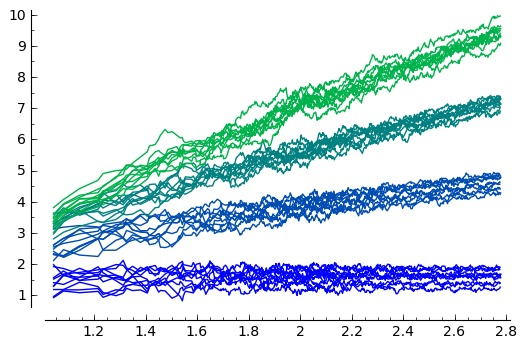
\includegraphics[width=0.7\textwidth]{bsd.jpg}
 \end{center}
 \caption{Oh look, something happens here !}
 \label{fig:bsd}
\end{figure}

\section{Conclusions} \label{sec:conclusions}

Further help on \LaTeX\ can be found easily on the internet. The \LaTeX\
wikibook\footnote{\tt http://en.wikibooks.org/wiki/LaTeX} contains a lot.
For instance you would find there how to type theorems and proofs nicely.
Or how to include source code written in some programming language like
python. There are long lists available with all sorts of common
mathematical symbols like $\xi$, $\nabla$, $\infty$, $\log$, $\iff$, etc.

\newpage

\appendix

\section{Raw data} \label{app:rawdata}

Material that needs to be included but would distract from the main
line of presentation can be put in appendices.
Examples of such material are raw
data, computing codes and details of calculations.

But note tha the maximal number of pages includes the appendix and the references.

\section{Calculations for section \ref{sec:my1}} \label{app:calculations}

In this appendix we could verify equation \eqref{eq:myeq1} or present the code that was used. 
\begin{lstlisting}[language=Python]
def gcd(a,b):
    """
    Return the greatest common divisor
    of a and b 
    """
    while b > 0:
        (a, b) = (b, a % b)
    return a
\end{lstlisting}

\newpage

\printbibliography

\end{document}
